\documentclass[11pt]{article}

\usepackage{threeparttable}
\usepackage{subfig}
\usepackage{pdfpages}
\usepackage{amsfonts,amsthm,amssymb,amsmath}
\usepackage{graphicx,mathrsfs}
\usepackage{multirow}
\usepackage{float}
%\usepackage{tikz}
%\usetikzlibrary{arrows}
% \usepackage[hidelinks=true]{hyperref}
% \usepackage{natbib}
% \bibliographystyle{chicago}
% page format
\usepackage[top=0.81in,bottom=0.81in,left=0.81in,right=0.81in%,a4paper
]{geometry}
\linespread{1.3}
\setlength{\parskip}{3.6pt}

%% for cross reference in paper
%\usepackage{hyperref}
%\hypersetup{colorlinks,citecolor=black,filecolor=black,%
%  linkcolor=black,urlcolor=black}

\newtheorem{thm}{Theorem}
\newtheorem{prop}{Proposition}
\newtheorem{assu}{Assumption}
\newtheorem{definition}{Definition}%[section]
\newtheorem{lemma}{Lemma}
\newtheorem{coro}{Corollary}
\newtheorem{example}{Example}
\newtheorem{fact}{Fact}
\newtheorem{conjecture}{Conjecture}
\newtheorem{alg}{Algorithm}
\newtheorem{rem}{Remark}
\newtheorem{fig}{Figure}

\newcommand{\rv}{random variable}
\newcommand{\bE}{\bf E}
\renewcommand{\Box}{\bigboxvoid}
\newcommand{\qeds}{$\qedsymbol $}
\newcommand{\R}{\mathbb{R}}
\newcommand{\Z}{\mathbb{Z}}
\newcommand{\cc}{\mathbb{c}}

 %Natbib setup for author-year style

\title{\textbf{Authors' Reply\\Lagrangian Heuristic for Simultaneous Subsidization and Penalization:\\
Implementations on Rooted Travelling Salesman Games}}
\author{Lindong Liu, Yuqian Zhou, Zikang Li}
\date{}

\begin{document}
\maketitle

\noindent

We would like to thank the Associate Editor for processing our submission efficiently and providing guidance for the revision, and also thank the Referees for the encouraging and detailed comments on the paper.
We have carefully studied all the comments and addressed them in our manuscript.

% In this reply, we summarize several major changes we have made, and then give the specific details.
%
% First, regarding the equality in (4) is replaced to >= inequality in (6), we add a more detailed explanation. Meanwhile we explain that LP(4) is not a restriction of LP(2) in Reply 1 to Referee 1, maybe the term 'restricted LP' on page 7 caused the misunderstanding and we now use 'variant' to replace 'restricted'.
%
% Second, regarding the upper bound $c_u(V)$, we forgot to mention how to obtain the upper bound.
% In fact, all the upper and lower bounds of $c(S)$ are obtained by the Lagrangian relaxation method to keep the consistency and continuity.
%
% Third, regarding the proofs of Theorem 1 and Remark 1, we now add a clarification on the negative cost allocation in Reply 3 to Referee 1 and another clarification on the meaning of "the point-wise maximum of a finite set of straight lines".
%
%
% Fourth, regarding the sub-gradient method, we add a detailed clarification on page 9 including how the initial values of Lagrangian multipiers are given and how they change during the sub-gradient method.
%
% Fifth, regarding the symmetry of TSP game and why the TSP game is defined on the complete graph in our manuscript, we make the corresponding explanation in Reply 8 and Reply 6.
%
% Sixth, regarding the Figure 2, we add the definitions of squared points and round points to the legend of the figure and the meaning of curves (a) and (c) in Figure 2 is explained on page 17.
%

Please find below our point-by-point reply to each of the Referees. To facilitate reading, the original comments are in {\it italics}.

%\vspace{10mm}
\newpage

\noindent \textbf{\large Reply to Referee 1}
\\[3mm]
We appreciate your detailed comments and clarification of your question.
We have carefully studied the technical concerns you raised, and revised our manuscript accordingly.

The main issues raised in your report are addressed as follows:
\\[4mm]
%
%
\noindent {\textbf{Question 1.}
However, my question focused on the LP (2) is as follows:
Is it true that in LP (2), one might replace constraint
$\beta(V) = c(V) - w$
by
$\beta(V) \geq c(V) - w$,
such that for any optimal solution to LP (2) this constraint will be binding?

$$\beta(S) \leq c_l(S) + z \leq c(S) + z$$
$$\beta(V) \textcolor{red}{\geq c_u(V) + z \geq c(V) + z}$$
{\small Note: According to your context, there may be some typos in your comments, and they are now revised in red.}

For example, it will become obvious that LP with constraints
$\beta(S) \leq c_l(S) + z \leq c(S) + z$
$\beta(V) \geq c_u(V) + z \geq c(V) + z$
will be the proper restriction of LP (2). Moreover, replacing c_l(S) and c_u(V) by c_u(S) and c_l(V)
$ \beta(S) \leq c_u(S) + z$
$ \beta(V) \geq c_l(V) + z$

\noindent \textbf{Reply 1.}
Thanks for your question. With regard to the conversion from the equality to the inequality, we have added more detailed explanations on page 9. For the second part of this question, we are sorry that the original term ``restricted LP" on page 7 is misunderstanding, and it is now replaced with term ``variant LP" to describe the relationships between LPs (2) and (4).

To be specific, when $c(S)$ and $c(V)$, in LP (2), are respectively replaced by $c_l(S)$ and $c_u(V)$ in LP (4).
Constraint $\beta(S) \leq c_l(S) + z \leq c(S) + z$ for any $S$ is a restriction of the original one, while $\beta(V) \geq c_u(V) + z \geq c(V) + z$ is not.
Therefore, LP(4) can be viewed as a variant, rather than a restriction, of LP(2).
Under the joint effects of the replacement of both constraints, we can find that LP(4) indeed can provide an upper bound for LP(2), as we have shown in Theorem 1.
\\[4mm]
%
%
%
\noindent {\textbf{Question 2.}
Other responses have not appeared clear to me either. For example, When I asked about upper bound on c(S) I am now referred to page 7, where it is stated that Lagrangian relaxation is used to find both bounds. How can Lagrangian relaxation be used to find both bounds? In any case, I have not seen any discussion about possible ways to obtain the upper bound c_u(V) and have not noticed the exact choice of the upper bound employed in the computational study.
~\\[2mm]

\noindent \textbf{Reply 2.}
Thanks a lot for your suggestion.
In the first half of this manuscript, we are trying to introduce a general framework of computing feasible subsidy-penalty pairs under which the grand coalition is stabilized.
Therefore, the upper bound $c_u(V)$ in LP(4) could be any value larger than $c(V)$.
It could be either named by some authority, or computed by some well known heuristic algorithm (such as the linear relaxation based heuristics).
In the second half of this manuscript, when the Lagrangian relaxation technique is applied for approximation, $c_u(V)$ is obtained by a Lagrangian relaxation based heuristic for the sake of consistency and generality. We have added this clarification on page 7.
% In fact, there are specific methods, such as LP-based methods, which can be used to obtain the upper bound $c_u(V)$.
% We have explicitly mentioned this in the paper.
% In order to be consistent with the general methods, we only mentioned a general method, i.e., Lagrangian heuristic to calculate the upper bound $c(V)$.
~\\[4mm]

\noindent {\textbf{Question 3.}
I am a bit confused by Figure 2. Does it represent 4 different games? What exactly is on y axis and x axis, Penalty and Subsidy on y and x axis for all 4 figures? I suggest to add definitions of squared points and round points to the legend of the figure. Why is it that one figure gets two points and another gets 6 and they are evaluated at different levels of subsidy?}
~\\[2mm]

The new clarification appeared on page 17 is still confusing. For example, 'the curve in subfigure (a) represents that the respective lines passing the two squared points have the same slope' -- I am not sure I understand how different lines can pass through two points, so the entire paragraph is confusing. Further on, I understand that the figure presents results for 4 different games. Why does a) instance obtain zero penalty-subsidy combinations, b) -- 1, c) -- 3, d) -- 4 combinations, what is the logic behind this?

\noindent \textbf{Reply 3.}
Thanks for your suggestions.
We are sorry for not making ourselves clear:
Figure 2 presents four representations of the curves of Lagrangian SPFs. The $x$ axis and the $y$ axis respectively represent the amount of subsidy and the amount of penalty in all 4 subfigures. We have added the definitions of squared points and round points into the legend of the figure.

\begin{figure}[H]
\centering
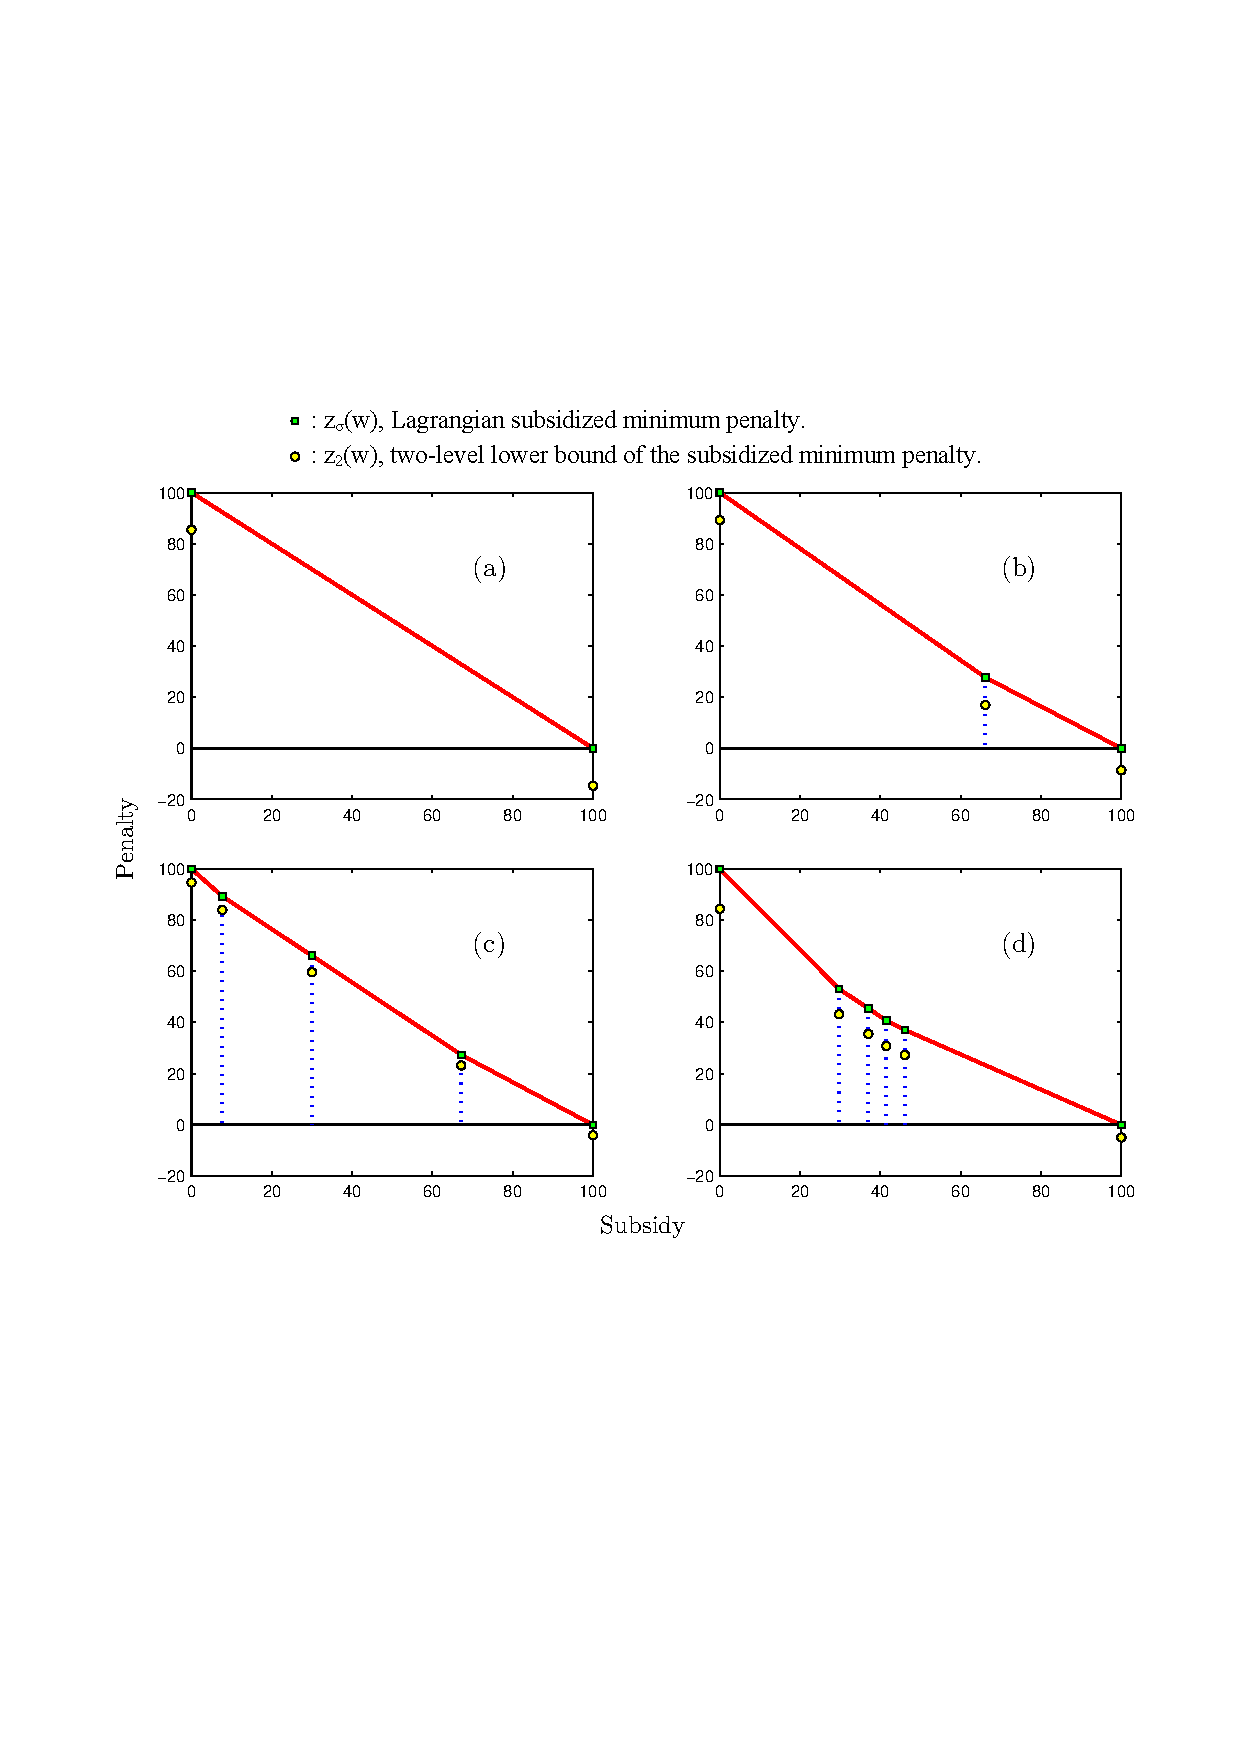
\includegraphics[width=1\textwidth]{1.pdf}
%\captionsetup{font={small}}
\centering
% \caption{\label{figure:20partitioned}Four representative Lagrangian SPFs for TSP games with 20 cities}
\end{figure}

In addition, the meaning of curves in subfigures (a) and (c) of Figure 2 is explained on page 17.
And the meaning of all curves in Figure 2 is shown below. The curve in subfigure (a) represents that the respective lines passing the two squared points have the same slope, thus there is no breakpoint between them.
% (a) represents that the slopes at the two points are equal, thus there is no breakpoint between them.
The curve in subfigure (b) represents that the two lines passing the two squared endpoints meets a point, besides, the value of $z_\theta(\omega)$ at x-coordinate value of the point is just equal to the value of y-coordinate of the point which indicates that this point is a breakpoint, which is the middle squared one. The curve in subfigure (c) represents that the two lines passing the two squared endpoints intersects a point under the third squared point. (Until here , we have not got the third squared point, but we know they have the same x-coordinate value.) Then with x-coordinate value of this intersection point, the third squared point can be obtained by Algorithm 1 in our manuscript. With the IPC algorithm proposed by Liu et al. (2018), we can generate a line passing the third squared point. Finally, this line intersects the two lines we mentioned at the beginning at the second and fourth squared points, respectively.
% (c) represents that the two lines passing the two points at the beginning and the end meets a point whose y-coordinate value is not equal to the third squared point's y-coordinate value, $z_\theta(\omega)$ at x-coordinate value of the point. The line passing the third squared point intersects the two lines passing the two points at the beginning and the end at the second and fourth squared points, respectively.
As for the curve in subfigure (d), the only difference between the curve in (c) and the curve in (d) is that the curve in (d) has one more line intersection process than that in (c) at the right half part of the subfigure.
~\\[4mm]

\noindent {\textbf{Question 4.}
The symmetry of TSP game. I would like to attract the attention of the authors to the Dantzig Fulkerson Johnson (1954) paper, which originated the development of the TSP theory. Most importantly, the authors there also considered a symmetric TSP problem. If the problem is symmetric, one does not need as many binary variables as was introduced by authors. For example, on page 13 $x_{ij}$ exists together with $x_{ji}$ but direction of the travel is not important for symmetric problem therefore it is sufficient to introduce $x_e$ for e being an edge or $x_{ij}$ for $i < j$ only. This is how the TSP problem was introduced in DFJ and this is something that can simplify many notations in this paper. Also, it will be probably a good idea to get rid of $x_{ii}$ variables on page 13 and other optimization problems.}
~\\[2mm]

I am still unclear why you introduce the symmetric TSP problems with the full set of binary variables $ x_{ij}, i = j$ instead of $x_{ij}, i < j$. This does not seem to be necessary in relation to coalitions S, please clarify.

\noindent \textbf{Reply 4.}
Thanks a lot for your comment.
Yes, as you have pointed out, when it comes to a symmetric TSP problem, it is more convenient to introduce decision variables such as $``x_e"$ or $``x_{ij}, i<j"$.
However, in the context of cooperative game theory (e.g., TSP game), since we have to indicate the existence of some player in a coalition (e.g., $\gamma^{S}_j=1$ indicates that player $j$ is in coalition $S$), it would be useful and neat to introduce variable $x_{ij}$ for better descriptions.
\\[4mm]


\noindent \textbf{Reply to Minor Comments.}
Thank you very much for pointing out the typos of our manuscript in Minor Comments. We have made corresponding revisions.

1. page 10, lines 19-21, $s_1$ and $s_2$ should probably be corrected to $S_2$ and $S_2$
2. page 4, line 36: linear programming problems
3. page 5, line 5: program
4. page 12, line 17, please add space after min
5. page 13, line 43, why do you need the notation 't' in $c_t(S)$?
6. page 14, line 10-11, could you please clarify the phrase 'constraints (14) and (15) are redundant due to (12)'?
7. page 15, line 41, 55: s.t.

% 1. We have changed our expression use LP problem to avoid the confusion. according to the Minor comments
%
% 2. We've revised.
%
% 3. We have added the concave property before mentioning the sub-gradient method.

% 5. We've replaced (9) by 'reduced cost' to avoid the forward reference.
%
% 6. We've added a reference to the Dantzig Fulkerson Johnson (1954) paper when introducing constraints (13).
%
% 7. We've merged the first two constraints for the ease of understanding.
%
% 8. We've removed the word 'minimum'.


%%%%%%%%%%%%%%%%%
\end{document}
%%%%%%%%%%%%%%%%%
